\documentclass[t]{beamer}

% Load general definitions
% Preamble file - general definitions, package loading, etc.

%=================================
% Load packages
\usepackage{amssymb,amsmath}
\usepackage{graphicx}
\usepackage{url}
\usepackage{tikz}
\usetikzlibrary{mindmap,trees,arrows}
\usepackage{fancyvrb}
\usepackage[portuguese]{babel} 
\usepackage[utf8]{inputenc}
\usepackage{subfigure}
\usepackage{times}
\usepackage[T1]{fontenc}
\usepackage{cancel}
\usepackage{color}
\usepackage{listings}
\usepackage[document]{ragged2e}
\usepackage{physics}
\usepackage{amsmath}
\usepackage{tikz}
\usepackage{mathdots}
\usepackage{yhmath}
\usepackage{cancel}
\usepackage{color}
\usepackage{siunitx}
\usepackage{array}
\usepackage{multirow}
\usepackage{amssymb}
\usepackage{gensymb}
\usepackage{tabularx}
\usepackage{extarrows}
\usepackage{booktabs}
\usetikzlibrary{fadings}
\usetikzlibrary{patterns}
\usetikzlibrary{shadows.blur}
\usetikzlibrary{shapes}

%=================================
% Set mode
\mode<presentation>
{
	\usetheme{Madrid}
	\usecolortheme{structure}
	\useoutertheme{infolines}
	\setbeamercovered{invisible}
}

% Get rid of nav bar
\beamertemplatenavigationsymbolsempty

% Insert frame number at bottom of the page.
\usefoottemplate{\hfil\tiny{\color{black!90}\insertframenumber}} 

%=================================
% Define new commands

\newcommand\Real{{\mathbb{R}}}
%\newcommand{\vi}{\vspace{0.6\baselineskip}}
%\newcommand{\goodgap}{\hspace{\subfigtopskip}\hspace{\subfigbottomskip}}


% Equation environments
\newcommand{\beq}{\begin{equation}}
\newcommand{\eq}{\end{equation}}
\newcommand{\beqs}{\begin{equation*}}
\newcommand{\eqs}{\end{equation*}}
\newcommand{\beqn}{\begin{eqnarray}}
\newcommand{\eqn}{\end{eqnarray}}
% Bold variables
\newcommand{\mbf}[1]{\ensuremath{\mathbf{#1}}}
% Itemization
\newcommand{\bitem}{\begin{itemize}}
\newcommand{\eitem}{\end{itemize}}
\newcommand{\spitem}{\vskip 1em\item}
\newcommand{\bitems}{\begin{itemize}\item}
\newcommand{\benums}{\begin{enumerate}\item}
\newcommand{\eenum}{\end{enumerate}}
% color blocks
\newenvironment{colorblock}[2]{%
\setbeamercolor{block title}{#2}
\begin{block}{#1}}{\end{block}}
% Vertical spacing
\newcommand{\vone}{\vskip 1em}
\newcommand{\vhalf}{\vskip .5em}
% Frame environments
\newenvironment{ftst}[3][t]{%
\begin{frame}{environment=ftst,#1}
\frametitle{#2}
\framesubtitle{#3}}{\end{frame}}
\newenvironment{ftstf}[2]{
\begin{frame}[fragile,environment=ftstf]
\frametitle{#1}
\framesubtitle{#2}}{\end{frame}}
% colors
\definecolor{MyGray}{rgb}{0.5,0.5,0.5}
\definecolor{MyDBGray}{rgb}{0.1,0.1,0.4}
\definecolor{darkgreen}{rgb}{0,0.4,0}
\definecolor{black}{rgb}{0,0,0}
\def\defn#1{{\color{red} #1}}
% Footnote
\renewcommand{\thefootnote}{\alph{footnote}}
% Relaxed footnotes
\newcommand{\lfr}[1]{\let\thefootnote\relax\footnote{\tiny #1}}
% Verbatim environment - using FANCYVRB package
\DefineVerbatimEnvironment%
{rcode}{Verbatim}
{fontsize=\scriptsize}
% Verbatim environment - using LISTINGS package
%\lstnewenvironment{rcode} {\lstset{	language = R,
%									basicstyle = \scriptsize\ttfamily,
%									showspaces = false,
%									showstringspaces = false,
%									showtabs = false,
%									keywordstyle = \color{black}\bfseries,
%									commentstyle = \color{darkgreen},
%									numbers = none,
%									otherkeywords={	<-,
%													ggplot,
%													geom_boxplot,
%													facet_grid,
%													shapiro.test,
%													fligner.test,
%													glht,
%													with},
%									deletekeywords={data,
%													model,
%													residuals,
%													c,
%													axis,
%													default,
%													labels,
%													qq.text}}}%
%{}

% Specific definitions
\title[]{Banco de dados II}
\subtitle[]{Transações}
\author[]{Patrícia Lucas\\{\footnotesize }}
\institute{Bacharelado em Sistemas de Informação \\ IFNMG  - Campus Salinas}
\date{\scriptsize Salinas\\Março 2022}

\begin{document}

% cover page
\setbeamertemplate{footline}{}
\begin{frame}

\begin{center}
\includegraphics[width=.15\textwidth]{}
\end{center}
  \titlepage
  \begin{tikzpicture}[remember picture,overlay]
  \node[anchor=south east,xshift=-5pt,yshift=5pt] at (current page.south east) {\tiny Versão 1.2021};
  \node[anchor=south west,yshift=0pt] at (current page.south west) {
\includegraphics[width=.25\textwidth]{Logos/salinas_horizontal_jpg.jpg}};
  \end{tikzpicture}  
\end{frame}

% Main slides

\begin{ftst}{Referência}{Transações}
\begin{figure}
    \centering
    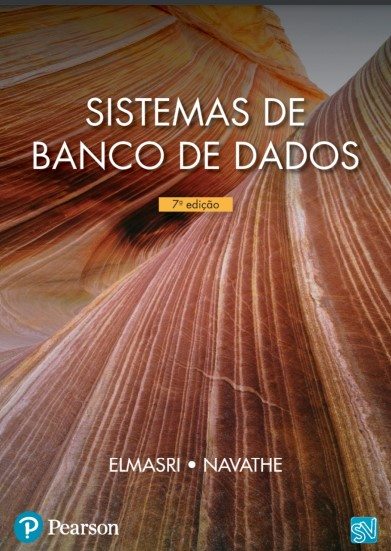
\includegraphics[scale=0.4]{Figuras/book.jpg}
\end{figure}
ELMASRI, R.; NAVATHE, S. B. Sistemas de Banco de Dados. 7. ed. São Paulo: Pearson Addison Wesley, 2019.
\end{ftst}

%==================================

\begin{ftst}{Visão geral}{Transações}

\begin{itemize}
    \item \textbf{Transação: } descreve uma unidade lógica de processamento em um Banco de Dados.
    \item \textbf{Sistema de Processamento de Transações: } 
    \begin{itemize}
        \item Precisam lidar com grandes Banco de Dados e milhares de usuários simultâneos.
        \item Requerem alta disponibilidade e tempo de resposta rápido.
    \end{itemize}
\end{itemize}
\end{ftst}

%==================================

\begin{ftst}{Processamento de Transações}{Transações}

\begin{itemize}
    \item \textbf{Transações atômicas: } unidade lógica de processamento em um Banco de Dados.
    \item \textbf{Controle de concorrência: } garantia de que múltiplas transações ativadas por vários usuários produzirão resultados corretos quando manipulam o banco de dados.
    \item \textbf{Recuperação de falhas: } garantia de que os efeitos das transações são mantidos no banco de dados mesmo com a ocorrência de falhas.

\end{itemize}
\end{ftst}

%==================================

\begin{ftst}{Monousuário versus Multiusuário}{Transações}

\begin{itemize}
    \item \textbf{SGBDs de monousuário:} no máximo um usuário de cada vez pode usar o sistema. 
    \item \textbf{SGBDs de multiusuário:} muitos usuários podem usar o sistema simultaneamente.
\end{itemize}
\end{ftst}

%==================================

\begin{ftst}{Multiprogramação versus Paralelismo}{Transações}

\begin{itemize}
    \item \textbf{Multiprogramação:} SO executa vários processos simultaneamente.
    \begin{itemize}
        \item Somente uma CPU.
        \item Preemptação: SO executa comandos de um processo, então suspende esse processo e executa comandos de outro processo, etc.
    \end{itemize}
    \item \textbf{Paralelismo:} várias CPUs disponíveis.
\end{itemize}

\begin{figure}
    \centering
    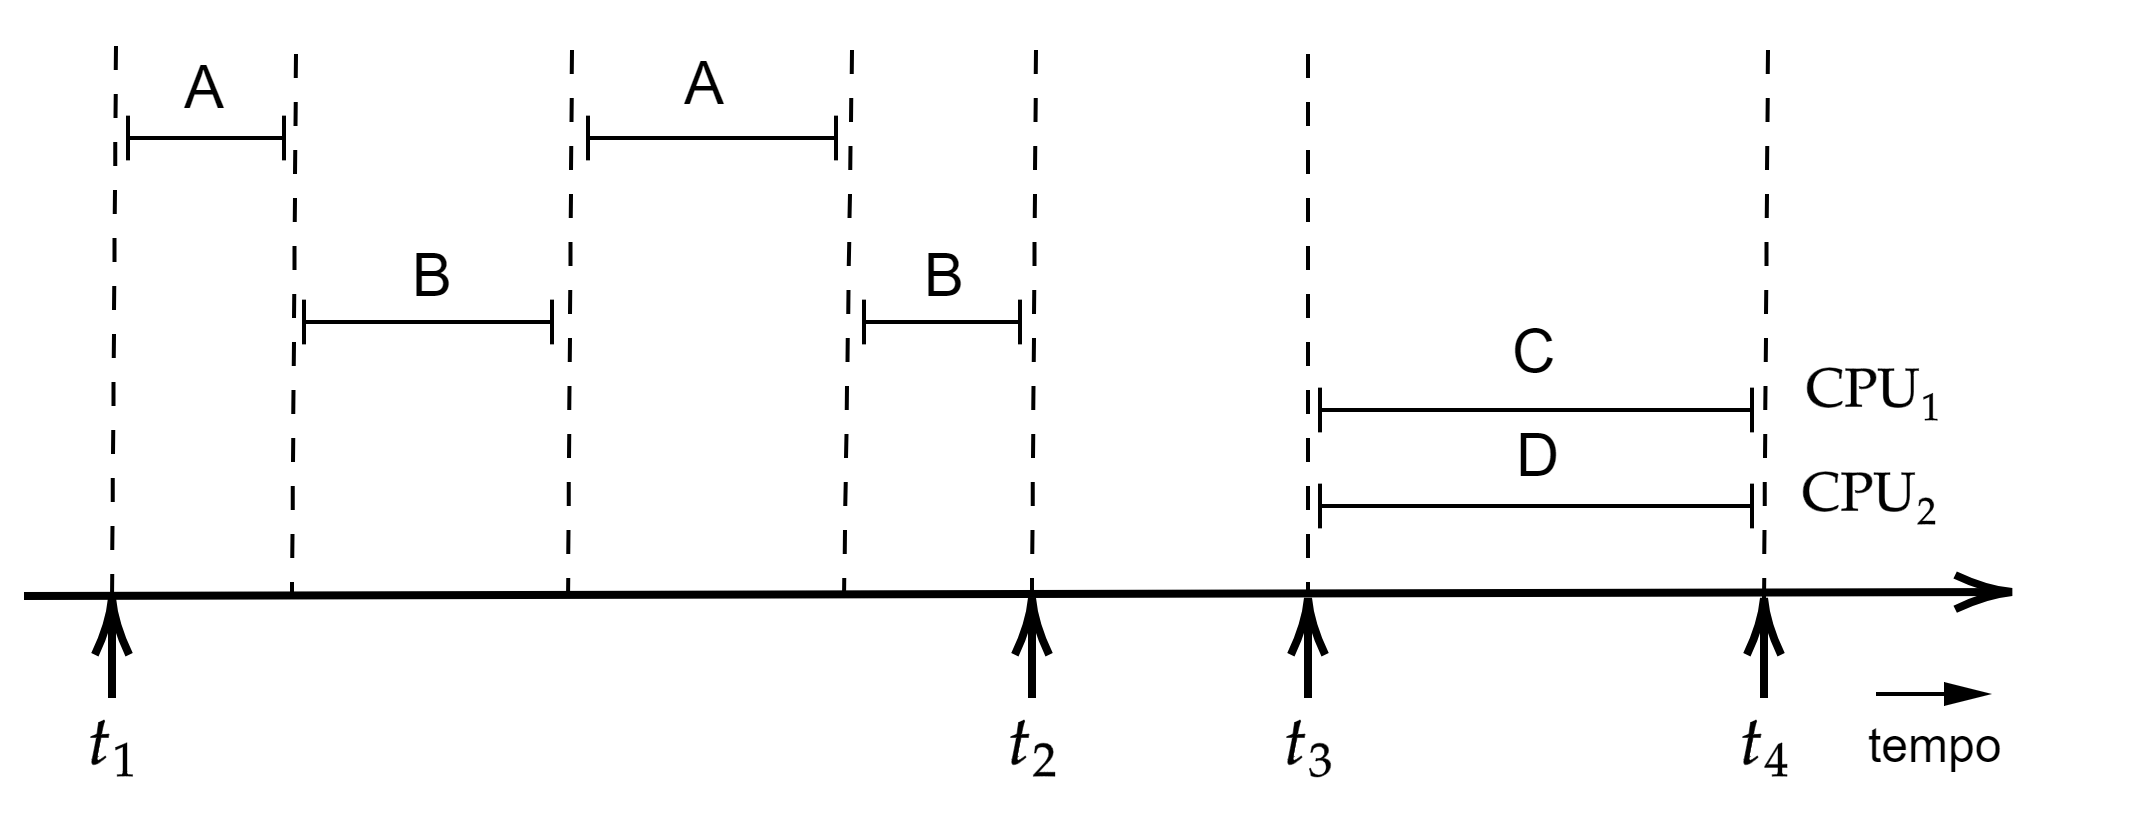
\includegraphics[scale=0.13]{Figuras_transacoes/1.png}
\end{figure}
\end{ftst}

%==================================

\begin{ftst}{Conceito de transação}{Transações}

Duas questões que devem ser levadas em consideração:
\vone
\begin{itemize}
    \item \textbf{Recuperação de falhas:} 
    \begin{itemize}
        \item Como lidar com falhas de vários tipos que ocorrem durante a execução das transações no SGBD.
        \item Falhas de hardware e falhas no sistema.
    \end{itemize}
    \item \textbf{Controle de concorrência:} 
    \begin{itemize}
        \item Execução simultânea de múltiplas de múltiplas transações.
        \item Transações concorrentes: acessam os mesmos itens de dados.
    \end{itemize}
\end{itemize}
\end{ftst}

%==================================

\begin{ftst}{Conceito de transação}{Transações}

\begin{itemize}
    \item Uma transação é uma unidade de execução de programa que acessa e possivelmente atualiza vários itens de dados.
    \item Exemplo:
\end{itemize}

\begin{figure}
    \centering
    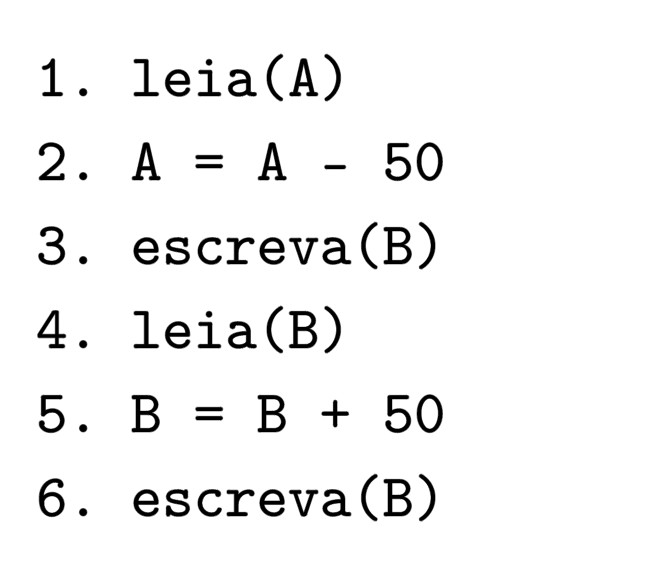
\includegraphics[scale=0.22]{Figuras_transacoes/2.png}
\end{figure}
\end{ftst}

%==================================

\begin{ftst}{Processamento de transações}{Transações}

\begin{itemize}
    \item \textbf{Modelo de transação:} 
    \vone
    \begin{itemize}
        \item READ\_ITEM(X): leitura de um item de dado X do banco de dados a ser armazenado em uma variável de programa.
        \item WRITE\_ITEM(X): escrita de uma variável de programa em um item de dados X do banco de dados.
    \end{itemize}
\end{itemize}
    \begin{figure}
        \centering
        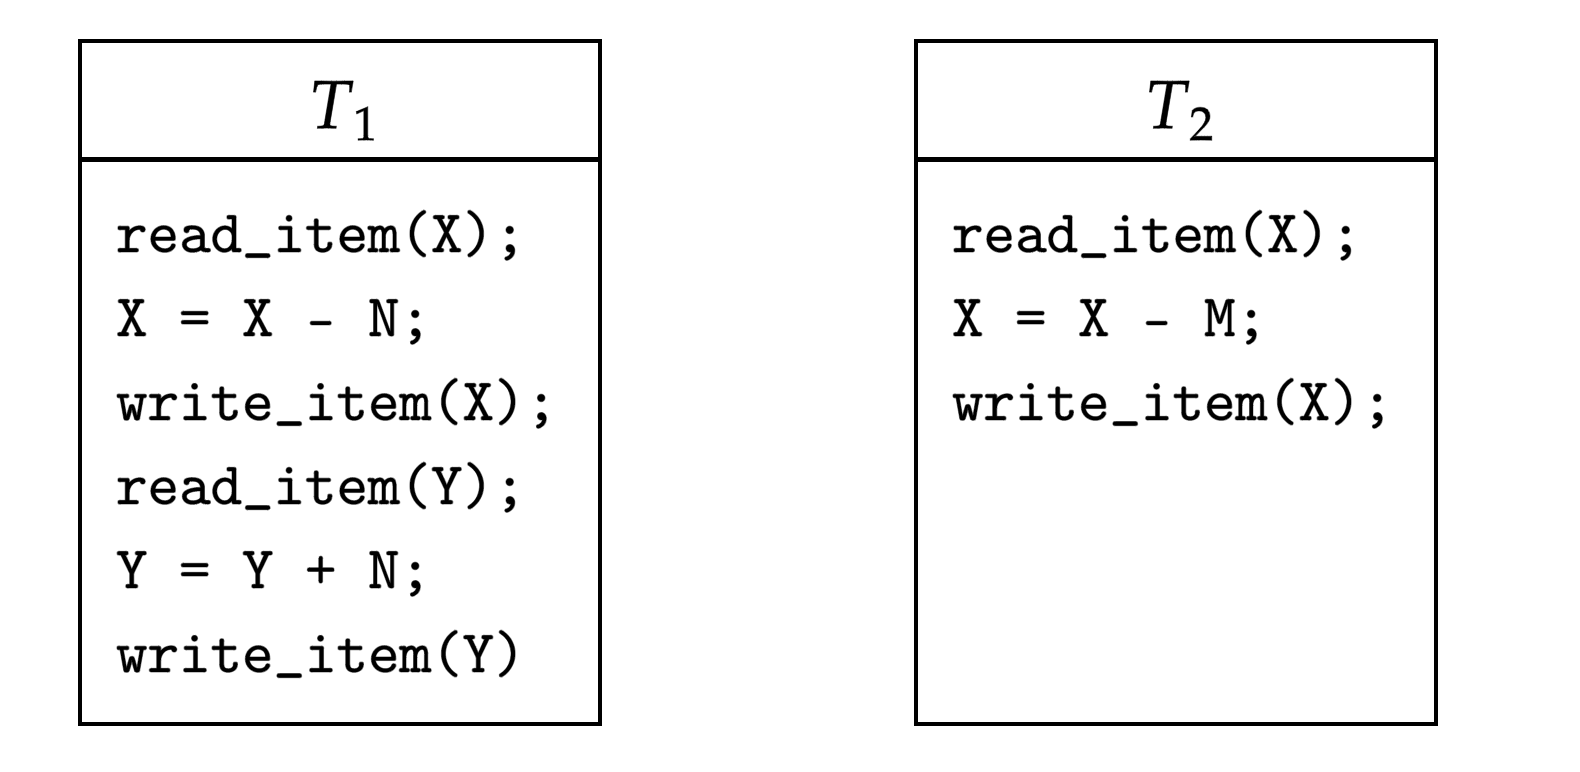
\includegraphics[scale=0.17]{Figuras_transacoes/3.png}
    \end{figure}
\end{ftst}

%==================================

\begin{ftst}{Itens de dados}{Transações}

\begin{itemize}
    \item \textbf{Granularidade:} tamanho de um item de dados. 
    \begin{itemize}
        \item Tupla.
        \item Bloco de disco.
        \item Valor de atributo de um registro.
    \end{itemize}
    \vone
    \item Conceitos de processamento de transações são independentes da granularidade do item.
\end{itemize}

\end{ftst}

%==================================

\begin{ftst}{Propriedades de uma transação}{Transações}

\begin{itemize}
    \item Para preservar a integridade dos dados, o SGBD deve garantir que cada transação siga as propriedades \textbf{ACID}.
    \vone
    \begin{itemize}
        \item Atomicidade.
        \item Consistência.
        \item Isolamento.
        \item Durabilidade.
    \end{itemize}
\end{itemize}

\end{ftst}

%==================================

\begin{ftst}{Propriedades de uma transação}{Transações}

\begin{itemize}
    \item \textbf{Atomicidade:} ou todas as operações da transação são devidamente refletidas no BD ou nenhuma está.
    \item \textbf{Consistência:} a execução de uma transação isoladamente preserva a consistência do BD.
    \item \textbf{Isolamento:} cada transação deve desconhecer outras transações de execução simultânea.
    \item \textbf{Durabilidade:} após a conclusão de uma transação, as alterações feitas no BD persistem, mesmo que haja falhas no sistema.
\end{itemize}

\end{ftst}

%==================================

\begin{ftst}{Propriedades de uma transação}{Transações}

\begin{itemize}
    \item \textbf{Atomicidade:} 
    \vone
    \begin{itemize}
        \item O SGBD deve garantir que as atualizações de uma transação parcialmente executada não sejam refletidas no BD.
        \item Exemplo de uma transferência bancária: se a transação falhar após 3, o dinheiro será perdido, levando a um estado inconsistente do BD. 
    \end{itemize}
\end{itemize}
    \begin{figure}
        \centering
        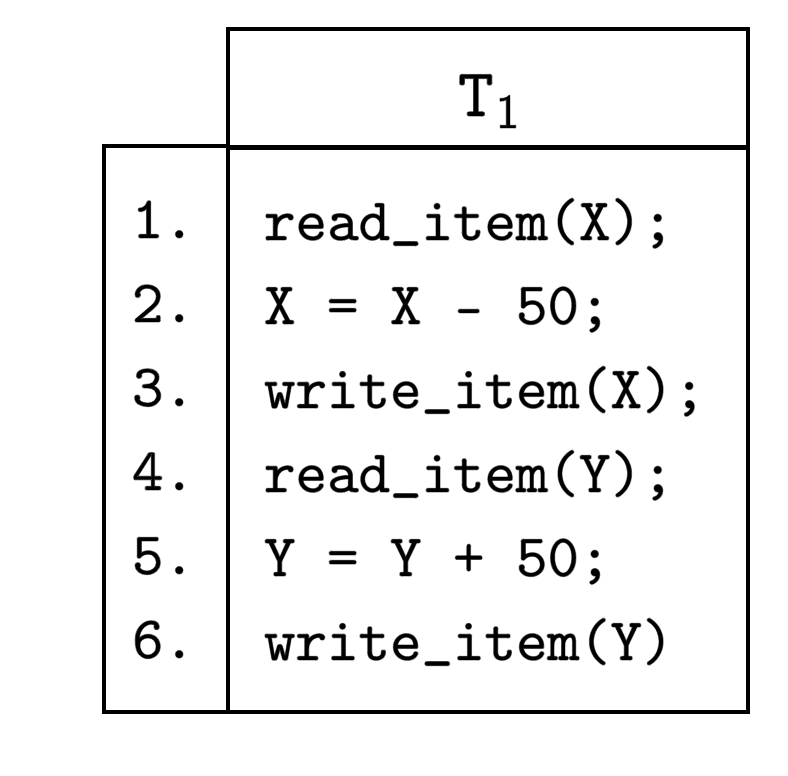
\includegraphics[scale=0.15]{Figuras_transacoes/4.png}
    \end{figure}
\end{ftst}

%==================================

\begin{ftst}{Propriedades de uma transação}{Transações}

\begin{itemize}
    \item \textbf{Consistência:} 
    \vone
    \begin{itemize}
        \item Uma transação deve preservar a consistência, significando que, se ela for completamente executada do início ao fim sem interferência de outras transações, deve levar o banco de dados de um estado consistente para outro também consistente. 
        \item \textbf{Causas:} violação das restrições de integridade, erro na semântica da transação, etc.
    \end{itemize}
\end{itemize}

\end{ftst}

%==================================

\begin{ftst}{Propriedades de uma transação}{Transações}

\begin{itemize}
    \item \textbf{Isolamento:} 
    \vone
    \begin{itemize}
        \item Uma transação deve parecer como se fosse executada isoladamente de outras transações, embora muitas delas estejam sendo executadas de maneira simultânea.
        \item A execução de uma transação não deve sofrer interferência de quaisquer outras transações que acontecem simultaneamente.
        \item Uma transação $T_1$ não pode ser dependente de outra transação $T_2$ que possa estar sendo executada ao mesmo tempo que $T_1$.
    \end{itemize}
\end{itemize}

\end{ftst}

%==================================

\begin{ftst}{Propriedades de uma transação}{Transações}

\begin{itemize}
    \item \textbf{Isolamento:} 
    \vone
    \begin{itemize}
        \item Exemplo de transações não isoladas:
    \end{itemize}
\end{itemize}
    \begin{figure}
        \centering
        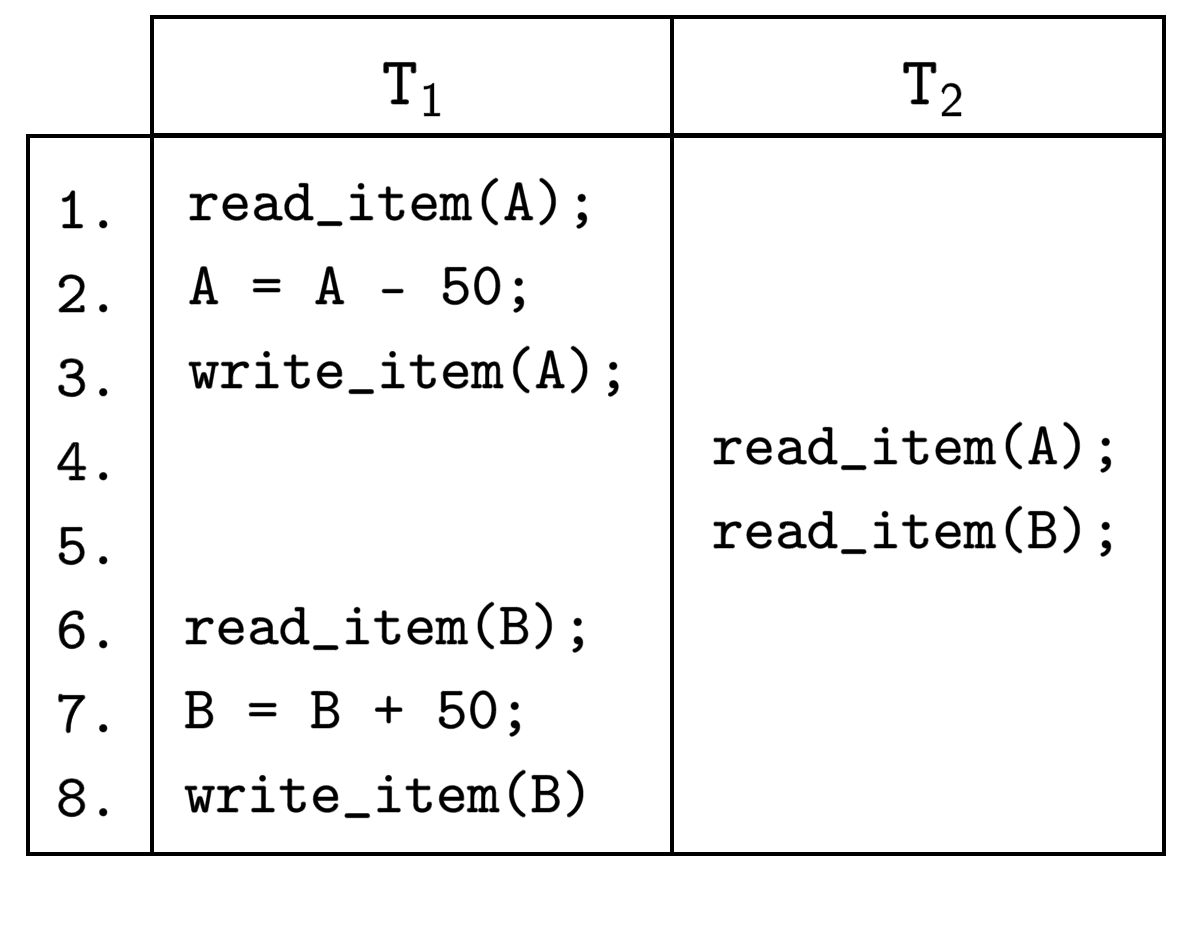
\includegraphics[scale=0.15]{Figuras_transacoes/5.png}
    \end{figure}

\end{ftst}

%==================================

\begin{ftst}{Propriedades de uma transação}{Transações}

\begin{itemize}
    \item \textbf{Durabilidade:} 
    \vone
    \begin{itemize}
        \item As mudanças aplicadas ao banco de dados pela transação confirmada precisam persistir no banco de dados. 
        \item Essas mudanças não devem ser perdidas por causa de alguma falha.
    \end{itemize}
\end{itemize}

\end{ftst}

%==================================

\begin{ftst}{Estados de uma transação}{Transações}
    \begin{figure}
        \centering
        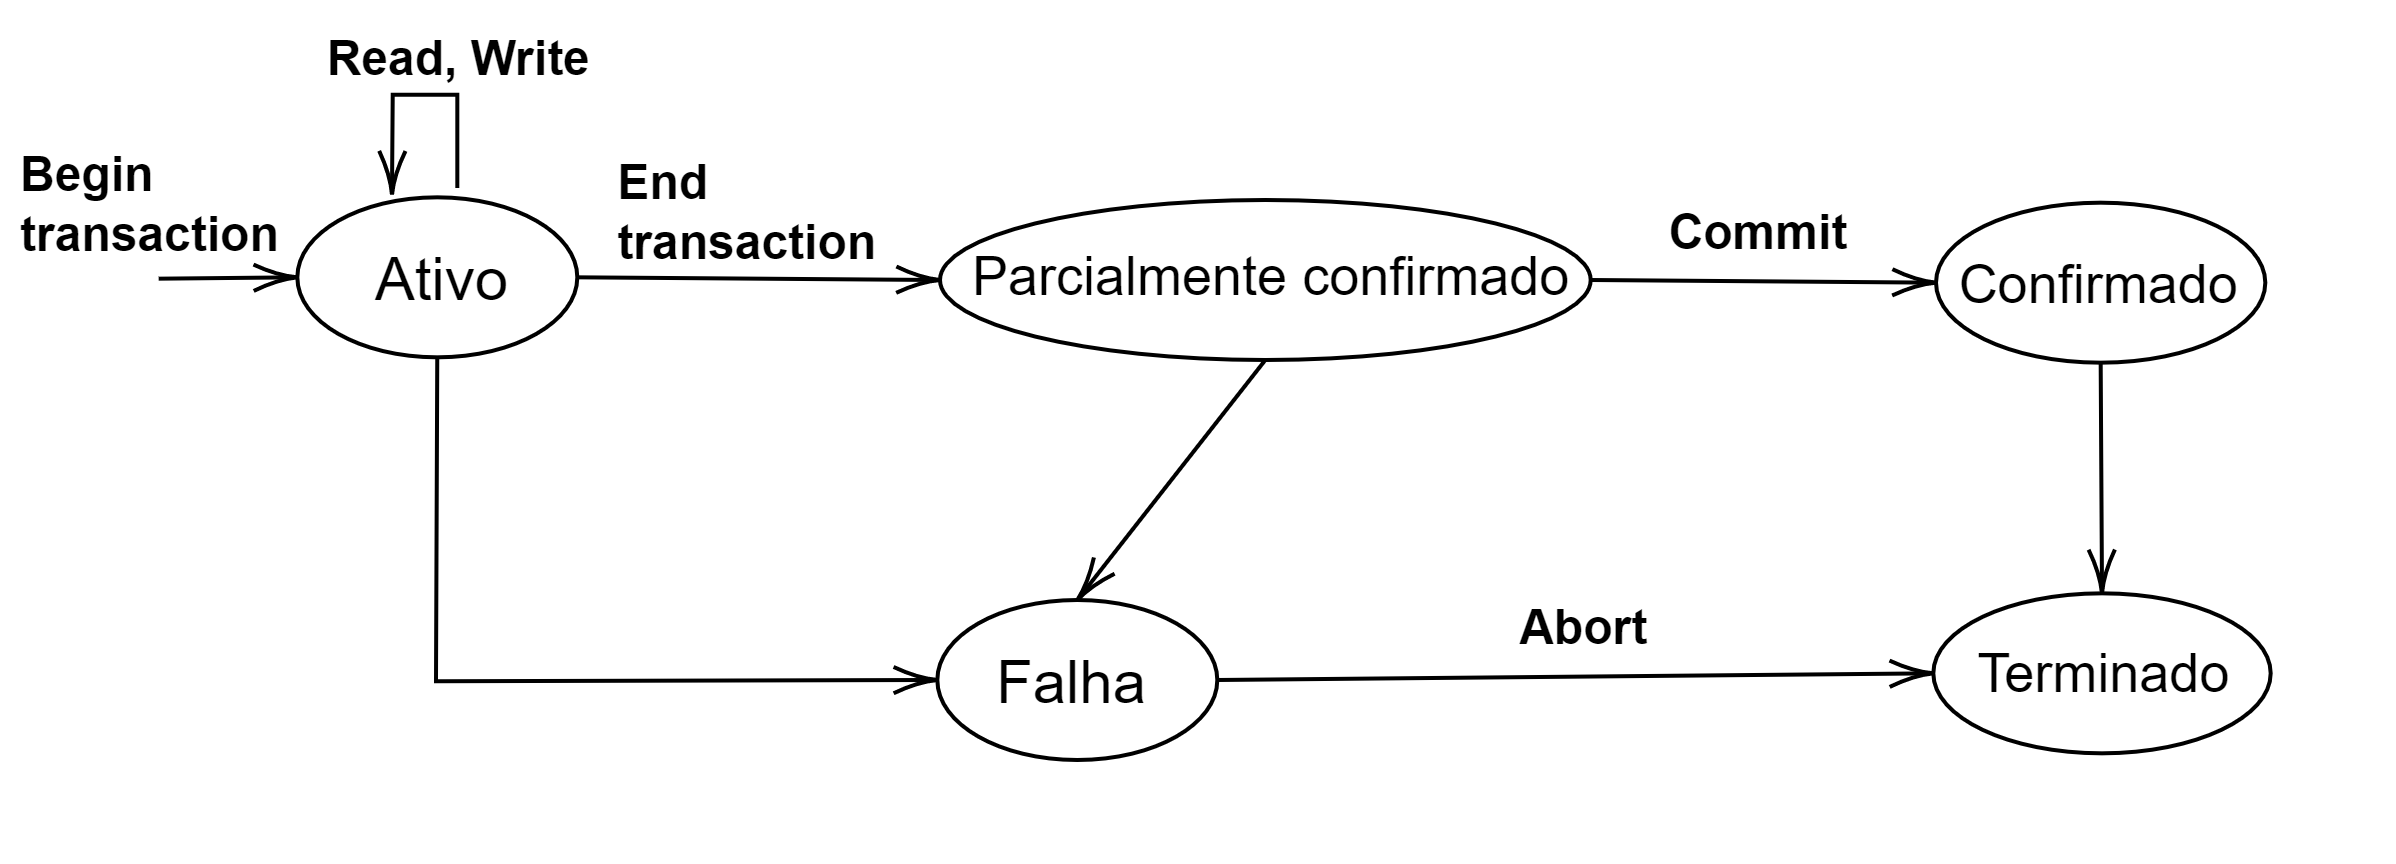
\includegraphics[scale=0.15]{Figuras_transacoes/6.png}
    \end{figure}
    \begin{itemize}
        \item \textbf{Ativo:} Uma transação entra em um estado ativo imediatamente após iniciar a execução, onde pode executar suas operações READ e WRITE.
    \end{itemize}
    
\end{ftst}

%==================================

\begin{ftst}{Estados de uma transação}{Transações}
    \begin{figure}
        \centering
        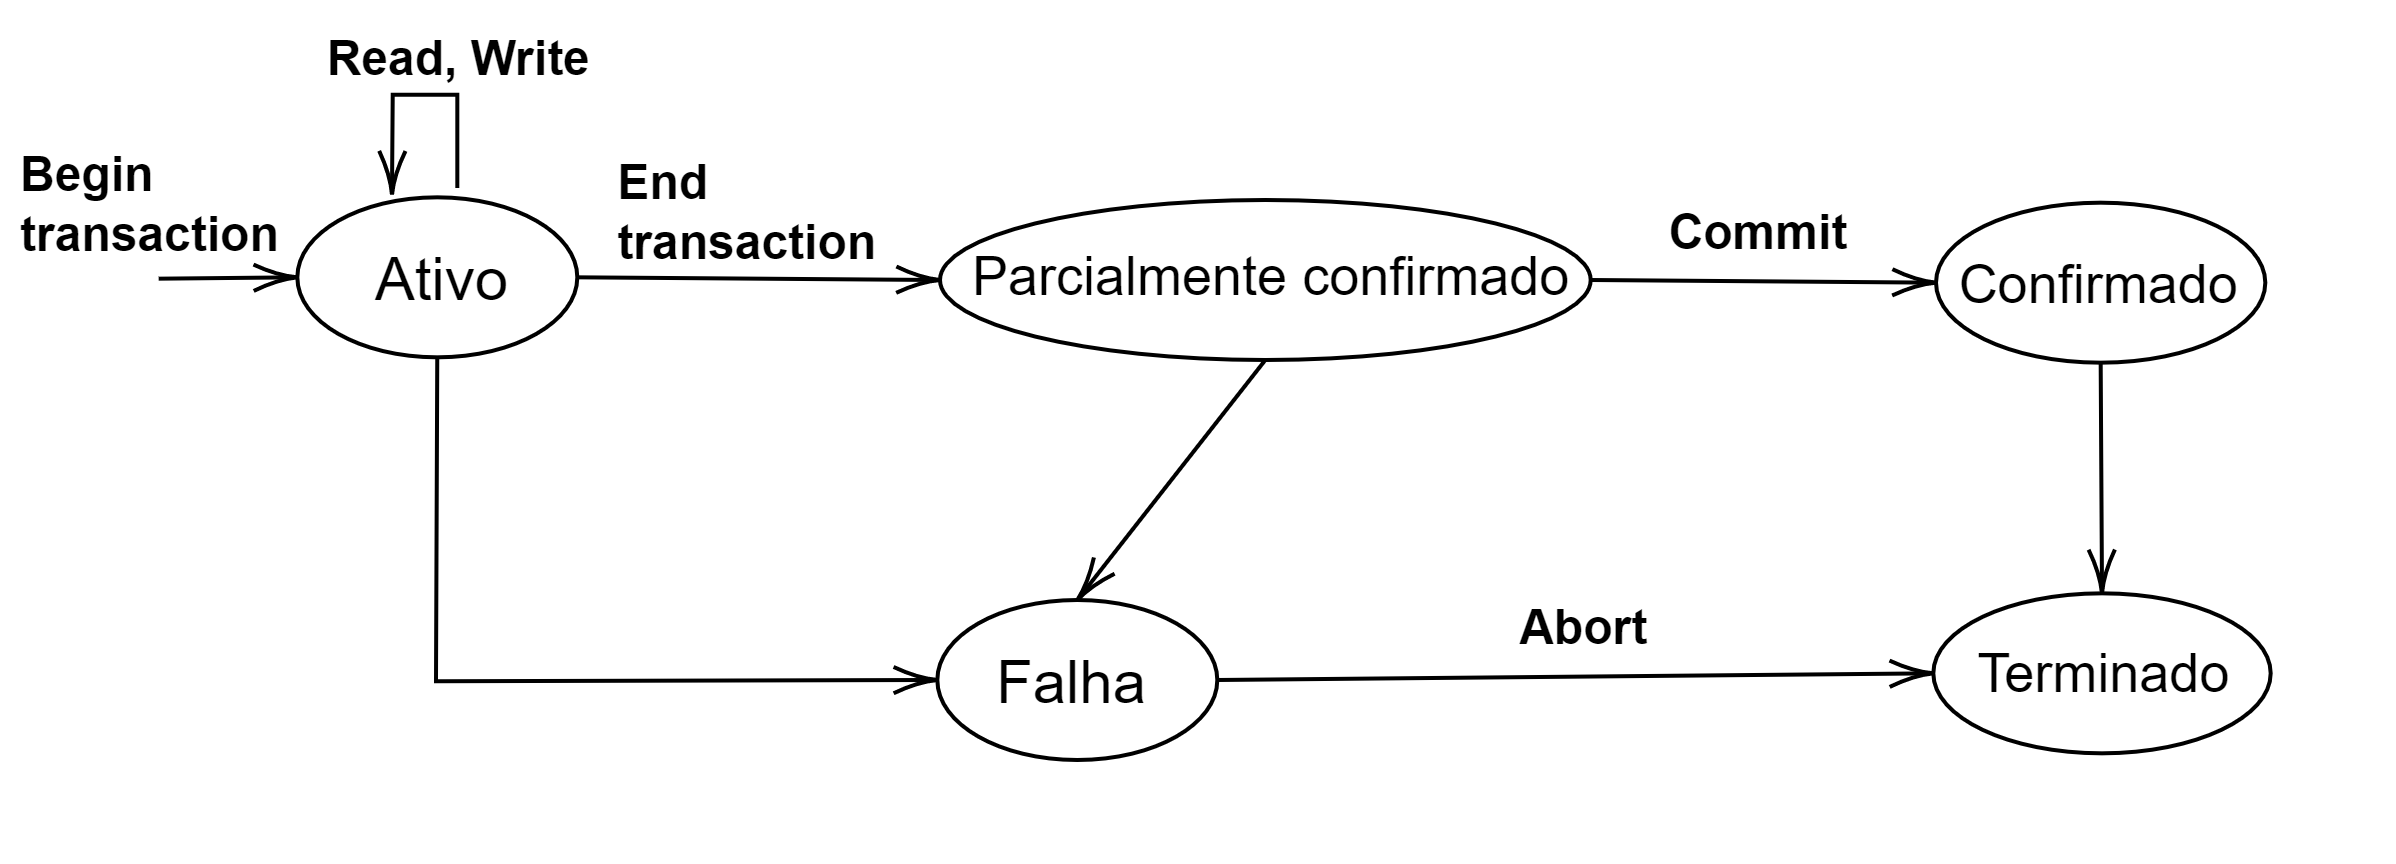
\includegraphics[scale=0.15]{Figuras_transacoes/6.png}
    \end{figure}
    \small
    \begin{itemize}
        \item \textbf{Parcialmente confirmado:} quando a transação termina. Nesse ponto, alguns protocolos de recuperação precisam garantir que uma falha no sistema não resultará em uma incapacidade de registrar as mudanças da transação permanentemente.
    \end{itemize}
    
\end{ftst}

%==================================

\begin{ftst}{Estados de uma transação}{Transações}
    \begin{figure}
        \centering
        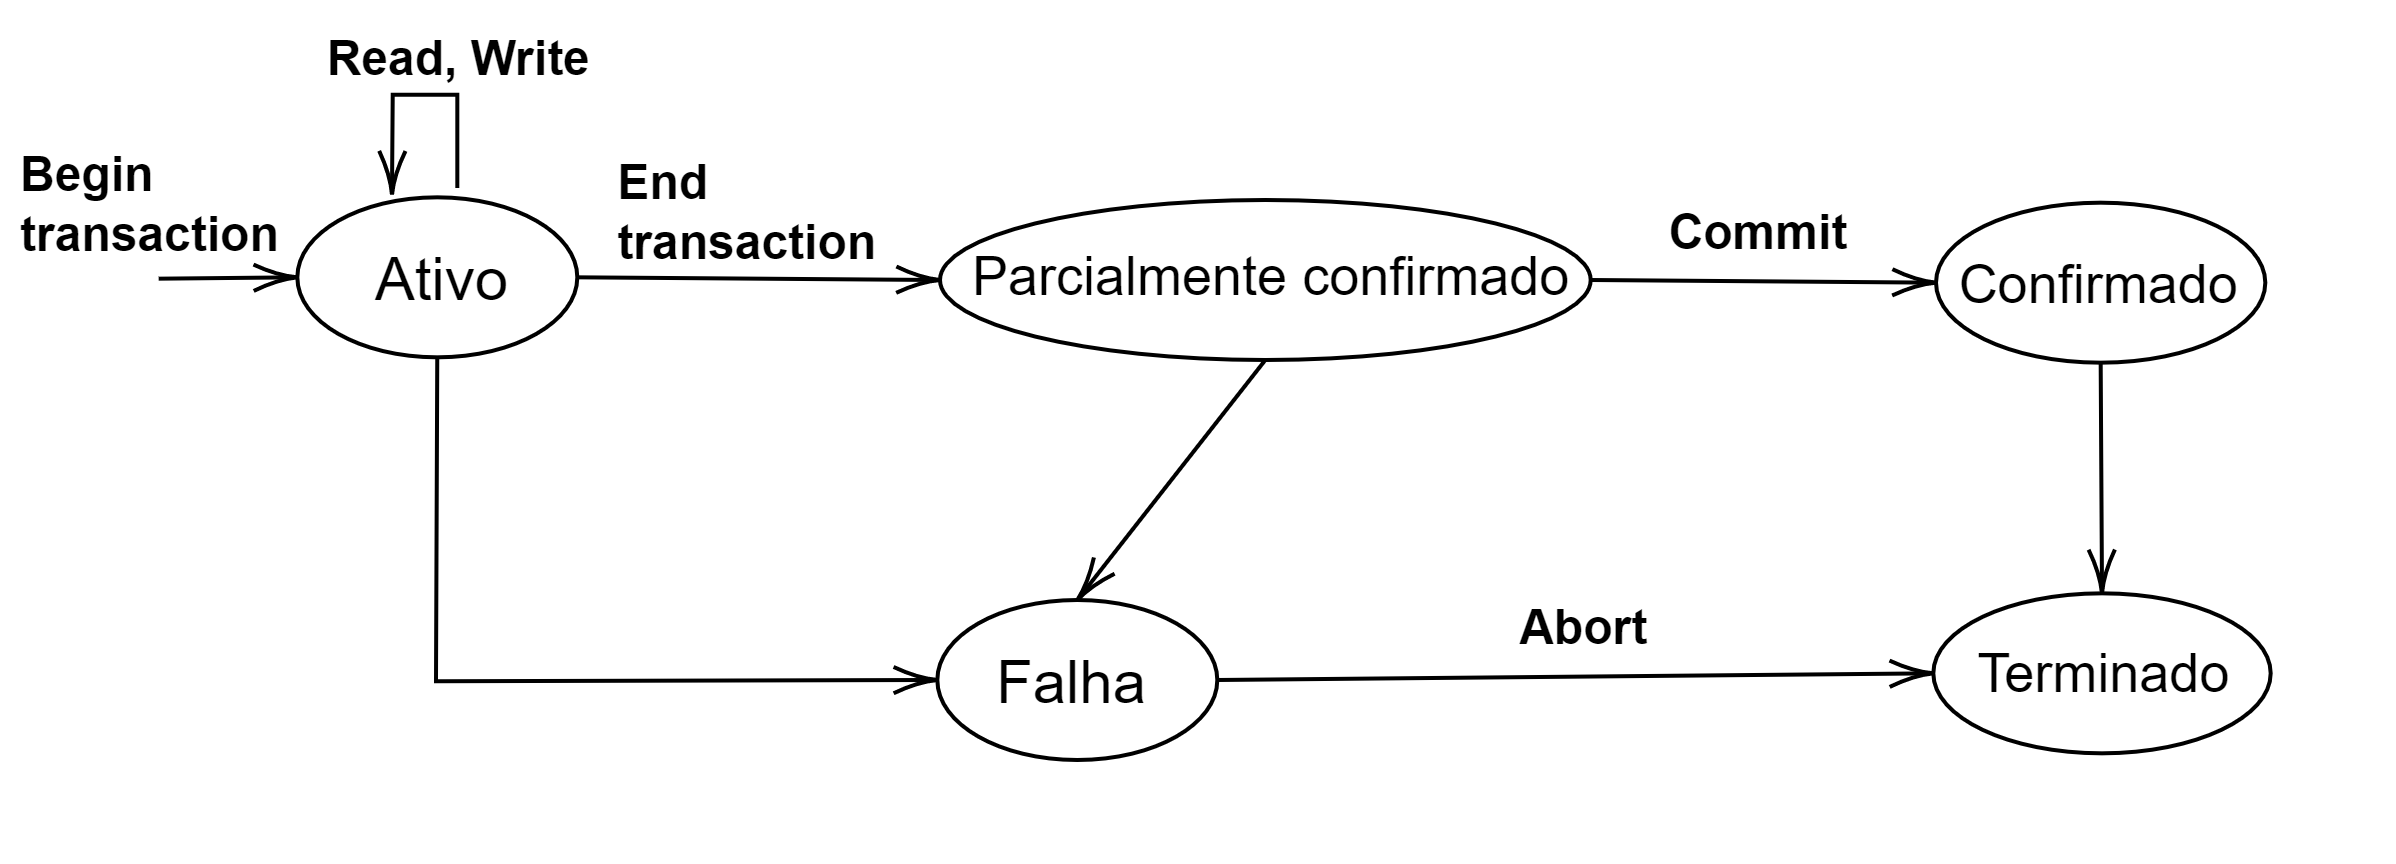
\includegraphics[scale=0.12]{Figuras_transacoes/6.png}
    \end{figure}
    \small
    \begin{itemize}
        \item \textbf{Confirmado:} Quando essa verificação é bem-sucedida, diz-se que a transação alcançou seu ponto de confirmação e ela entra no estado confirmado. 
        \item Quando uma transação é confirmada, ela concluiu sua execução com sucesso e todas as suas mudanças precisam ser gravadas permanentemente no banco de dados, mesmo que haja uma falha no sistema.
    \end{itemize}
    
\end{ftst}

%==================================

\begin{ftst}{Estados de uma transação}{Transações}
    \begin{figure}
        \centering
        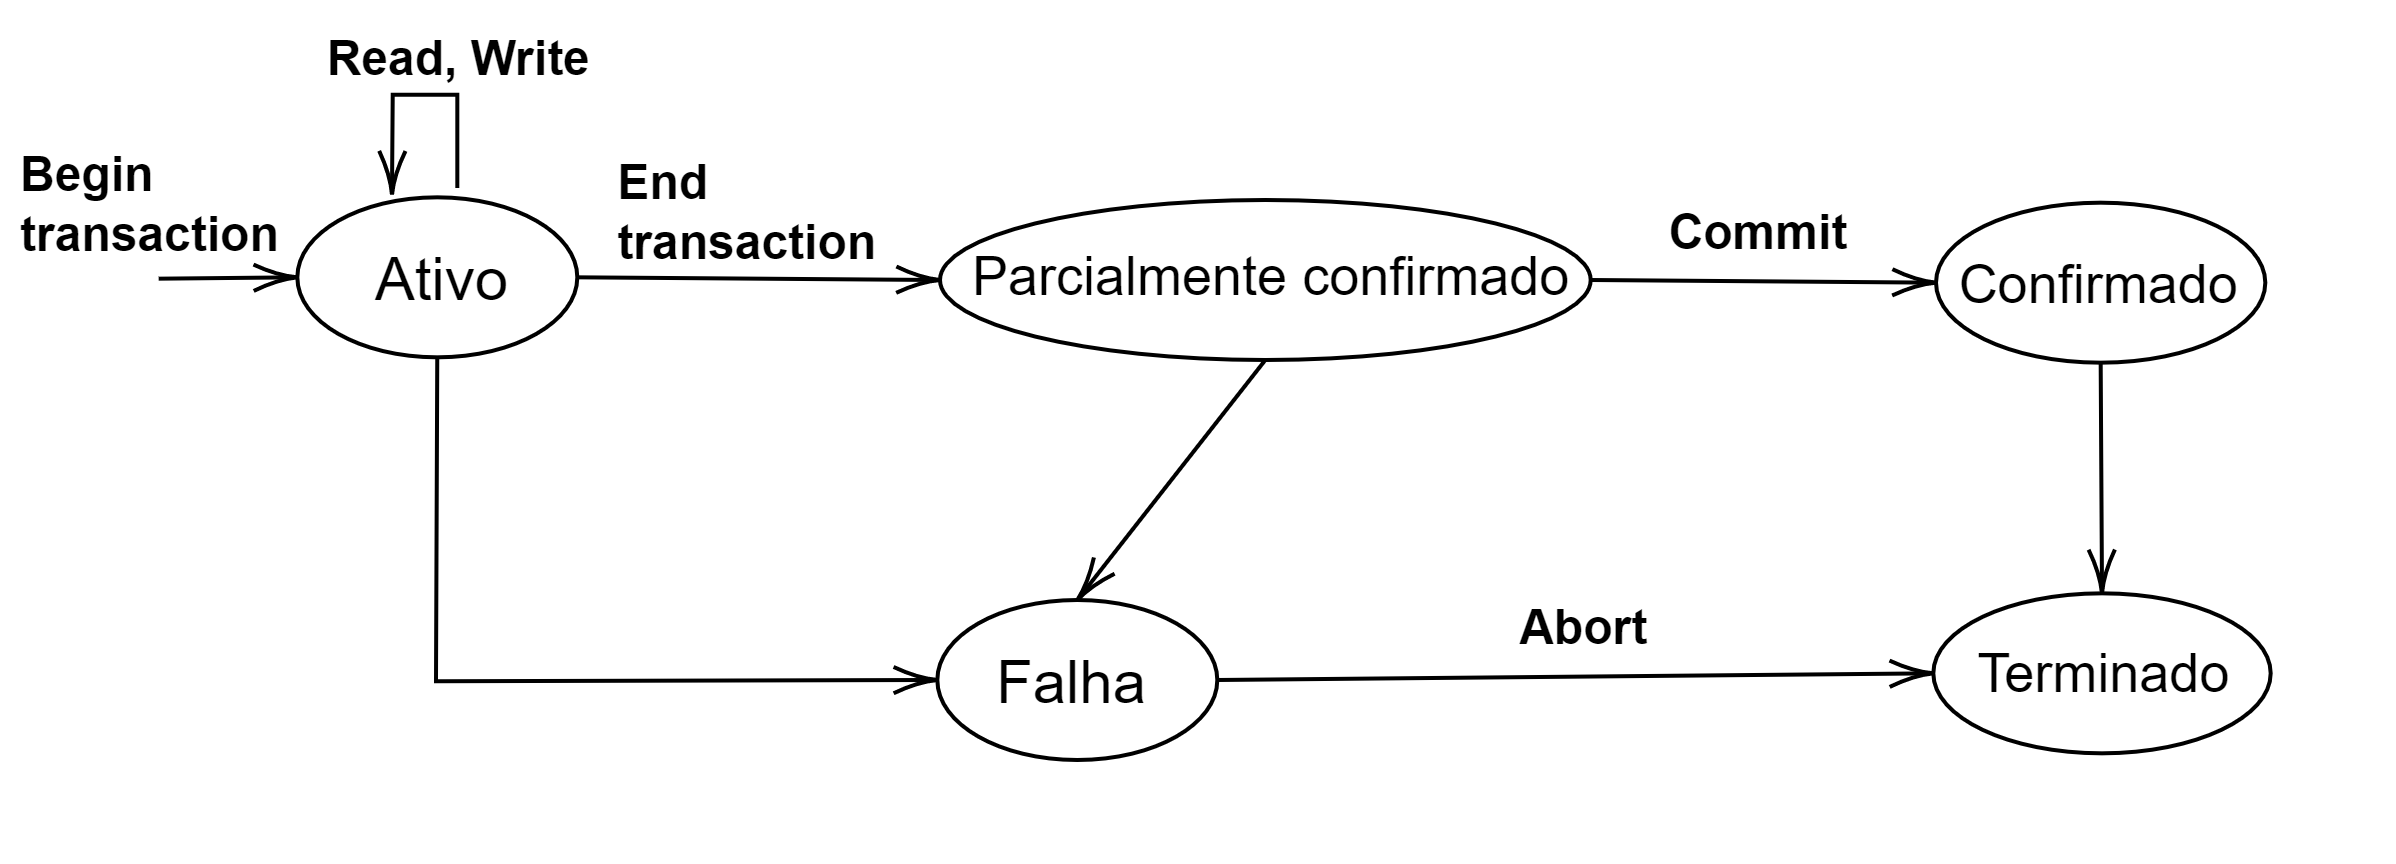
\includegraphics[scale=0.15]{Figuras_transacoes/6.png}
    \end{figure}
    \small
    \begin{itemize}
        \item \textbf{Falha:} se uma das verificações falhar ou se a transação for abortada durante seu estado ativo.
    \end{itemize}
    
\end{ftst}

%==================================

\begin{ftst}{Estados de uma transação}{Transações}
    \begin{figure}
        \centering
        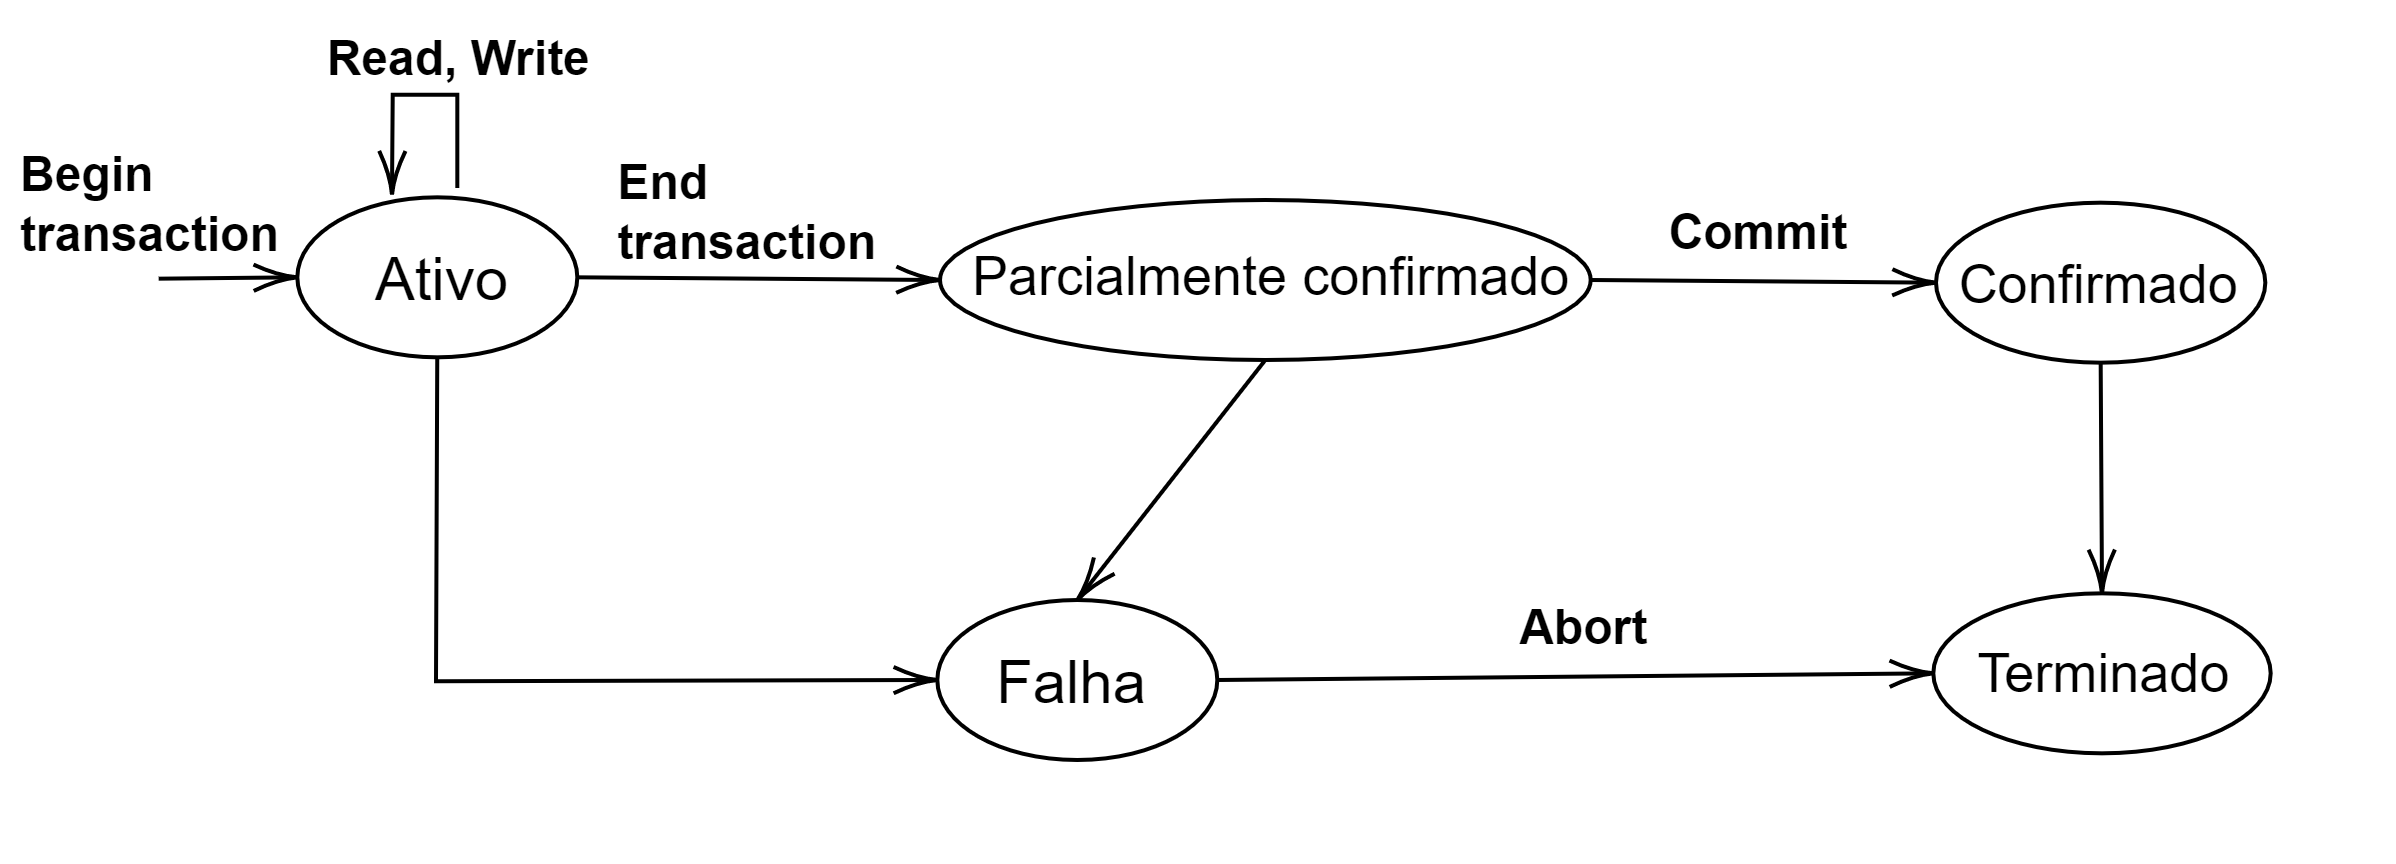
\includegraphics[scale=0.15]{Figuras_transacoes/6.png}
    \end{figure}
    \small
    \begin{itemize}
        \item \textbf{Terminado:} corresponde à transação que sai do sistema.
    \end{itemize}
    
\end{ftst}

%==================================

\begin{ftst}{Execuções Simultâneas de transações}{Transações}
\begin{itemize}
    \item Várias transações podem ser executadas simultaneamente no sistema.
    \item Vantagens:
    \begin{itemize}
        \item Melhor utilização de recursos: $T_1$ usa a CPU enquanto $T_2$ lê/escreve no disco.
        \item Tempo médio de resposta reduzido: transações curtas não precisam esperar por transações longas para serem processadas.
    \end{itemize}
\end{itemize}  
\end{ftst}

%==================================

\begin{ftst}{Controle de concorrência}{Transações}
\begin{itemize}
    \item Mecanismo de controle de concorrência são usados para alcançar o isolamento.
    \item Ou seja, controlar a interação entre as transações simultâneas, a fim de evitar que elas destruam a consistência do BD.
    \item Problemas que podem ocorrer quando as transações são executadas simultaneamente:
    \begin{itemize}
        \item Atualização perdida.
        \item Atualização temporária (leitura suja).
        \item Sumarização incorreta.
        \item Leitura não repetitiva (dupla):
    \end{itemize}
\end{itemize}  
\end{ftst}

%==================================

\begin{ftst}{Controle de concorrência}{Transações}
\begin{itemize}
    \item \textbf{Atualização perdida:} quando duas transações que acessam o mesmo item têm suas operações intercaladas de modo que isso torna incorreto o valor de alguns itens no banco.
\end{itemize}
\begin{figure}
    \centering
    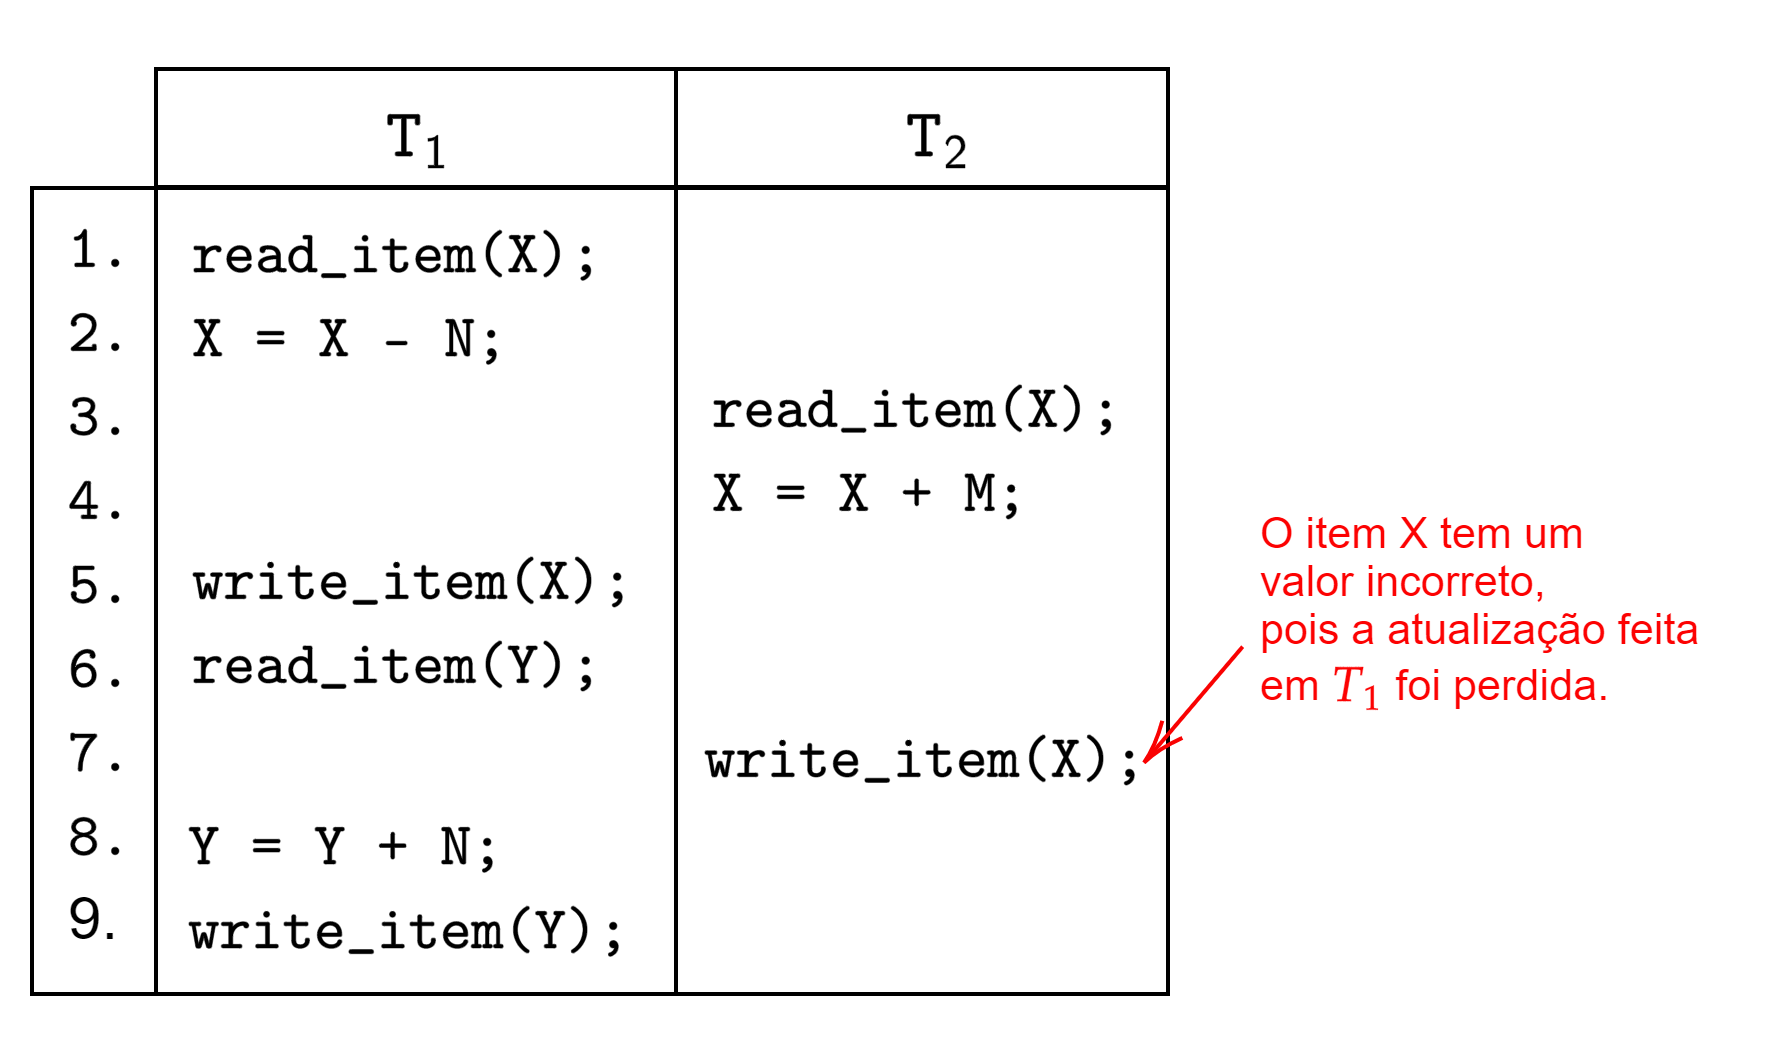
\includegraphics[scale=0.15]{Figuras_transacoes/7.png}
\end{figure}
\end{ftst}

%==================================

\begin{ftst}{Controle de concorrência}{Transações}
\begin{itemize}
    \item \textbf{Atualização temporária (leitura suja):} quando uma transação atualiza um item e depois falha. Nesse meio tempo, o item atualizado é acessado por outra transação, antes de ser alterado de volta para seu valor original.
\end{itemize}
\begin{figure}
    \centering
    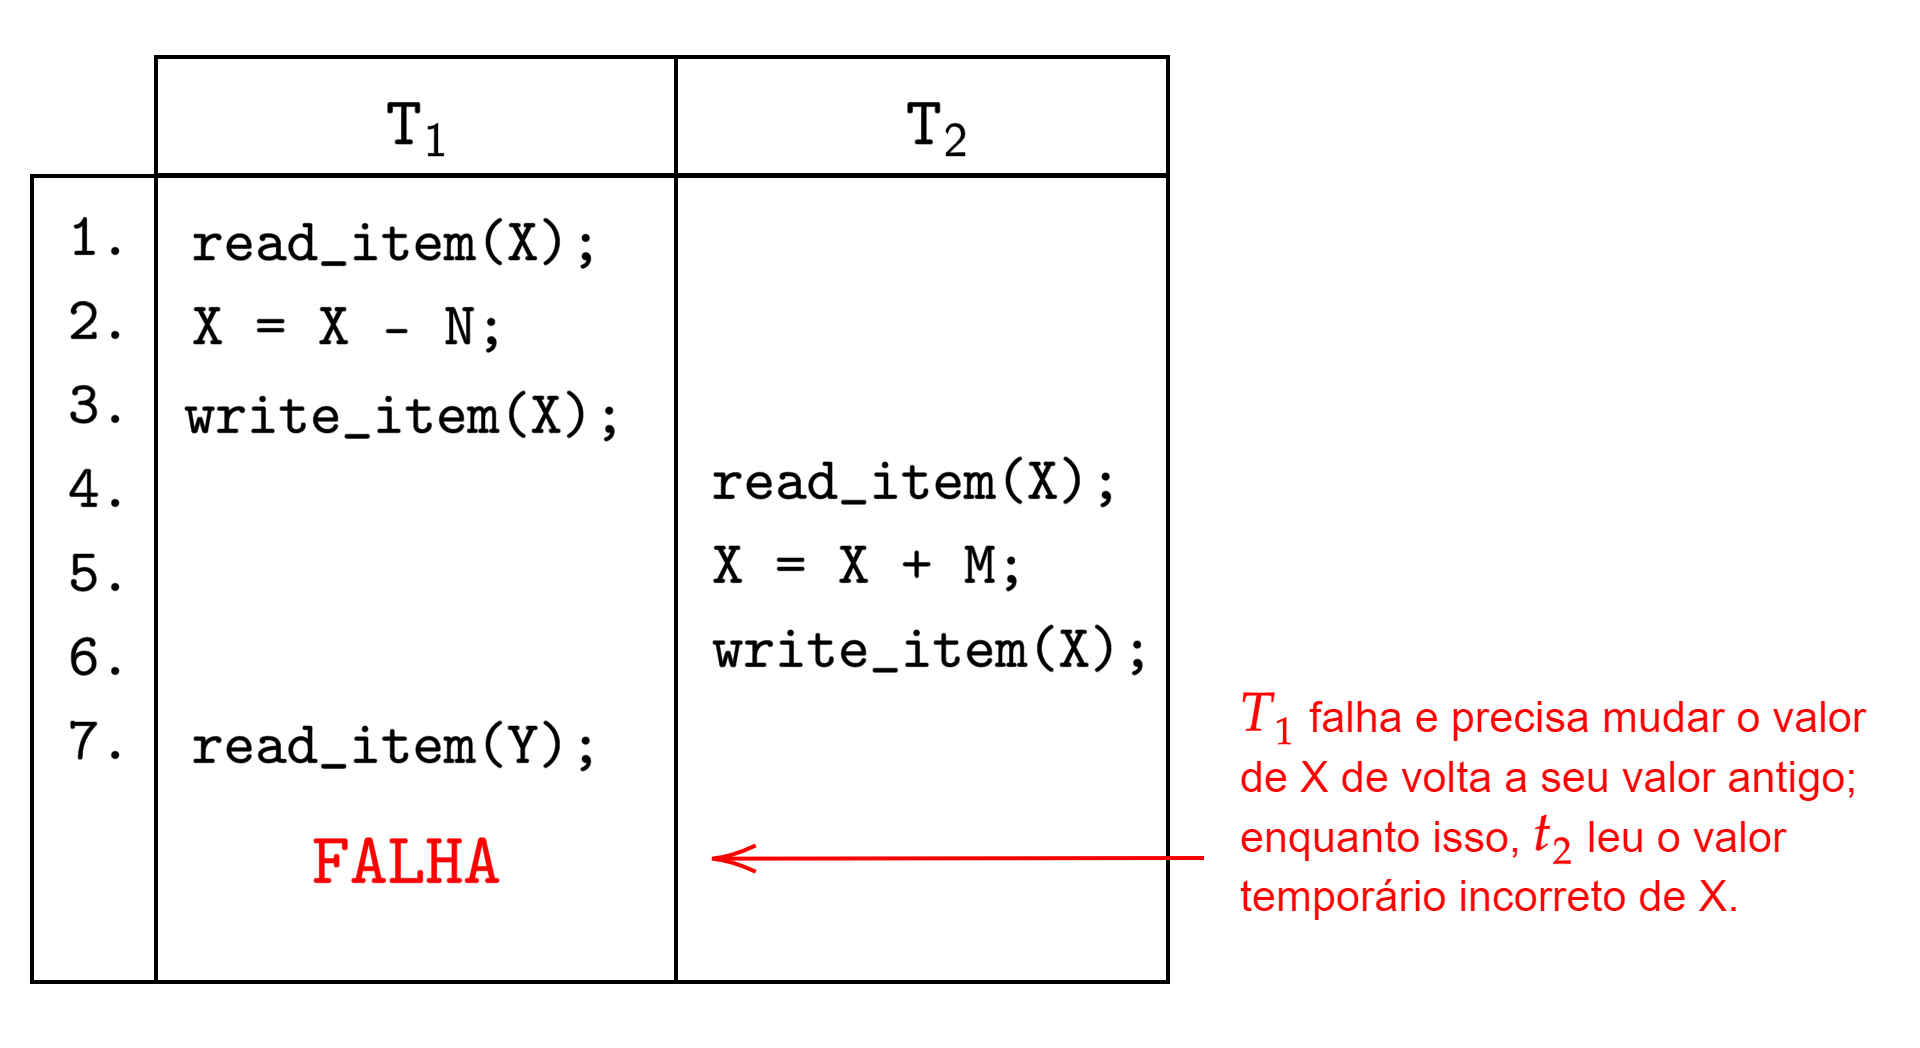
\includegraphics[scale=0.15]{Figuras_transacoes/8.png}
\end{figure}
\end{ftst}

%==================================

\begin{ftst}{Controle de concorrência}{Transações}
\small
\begin{itemize}
    \item \textbf{Sumarização incorreta:} se uma transação está calculando uma função resumo de agregação sobre uma série de itens, enquanto outras transações estão atualizando alguns desses itens, a função de agregação poderá calcular alguns valores antes de serem atualizados e outros depois de serem atualizados.
\end{itemize}
\begin{figure}
    \centering
    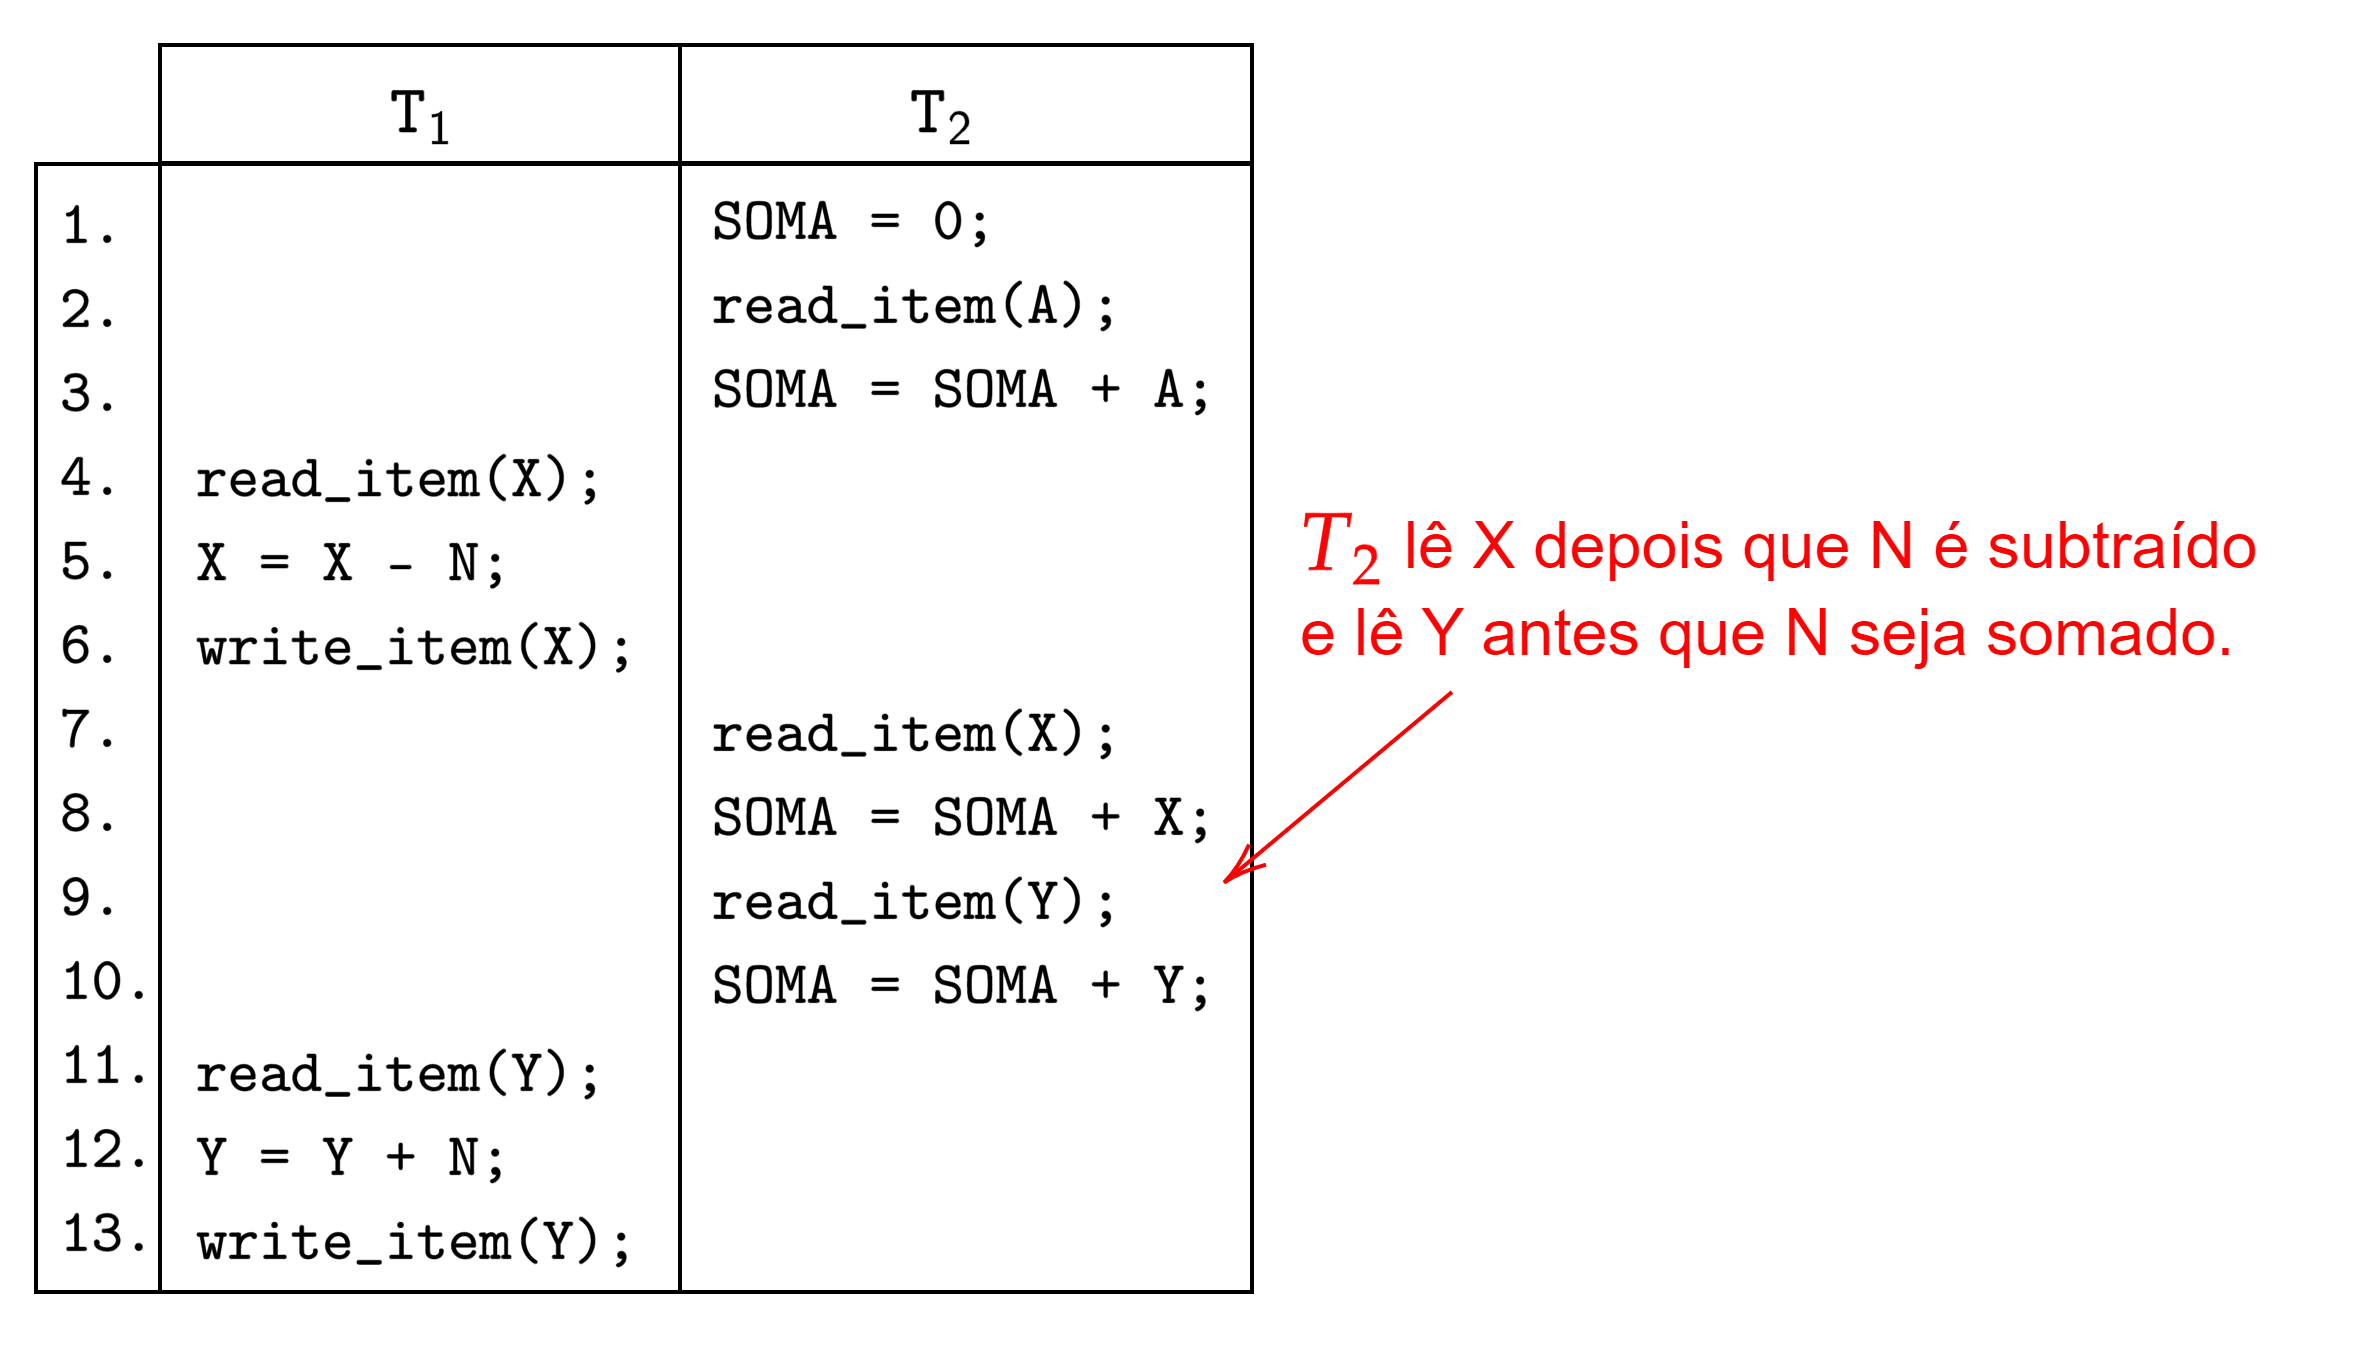
\includegraphics[scale=0.11]{Figuras_transacoes/9.png}
\end{figure}
\end{ftst}

%==================================

\begin{ftst}{Controle de concorrência}{Transações}
\begin{itemize}
    \item \textbf{Leitura não repetitiva (dupla):} ocorre quando uma transação $T_1$ lê o mesmo item duas vezes e o item é alterado por outra transação $T_2$ entre as duas leituras.
\end{itemize}
\begin{figure}
    \centering
    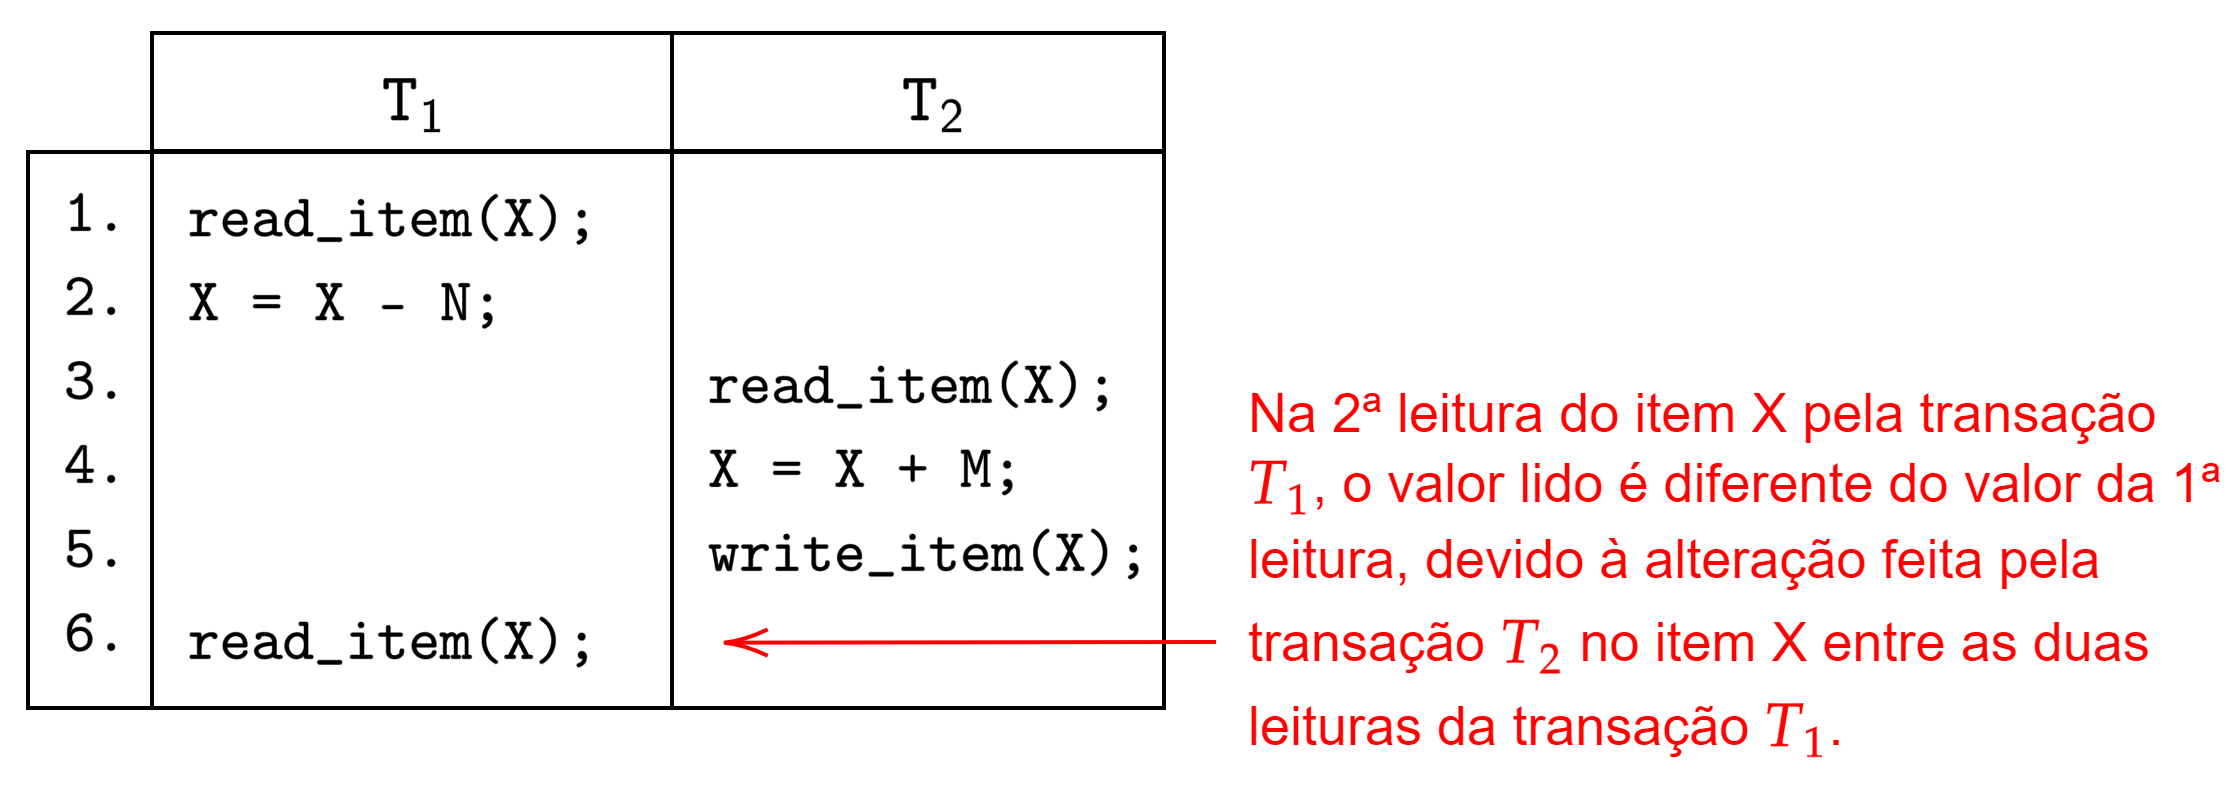
\includegraphics[scale=0.15]{Figuras_transacoes/10.png}
\end{figure}
\end{ftst}

%==================================

\begin{ftst}{Recuperação de falhas}{Transações}
\begin{itemize}
    \item Quando uma transação é submetida para execução em um SGBD, o sistema é responsável em garantir que:
    \vone
    \begin{itemize}
        \item todas as operações da transação serão completadas com sucesso e seus efeitos serão permanentemente registrados no BD; ou
        \item a transação não terá efeito no BD.
    \end{itemize}
\end{itemize}
\end{ftst}

%==================================

\begin{ftst}{Recuperação de falhas}{Transações}
\begin{itemize}
    \item Tipos de falhas:
    \begin{itemize}
        \item Falhas de sistema de computação - hardware/software.
        \item Erro na transação: erro lógicos, de programação, divisão por zero, etc.
        \item Erro locais ou condições de exceção na aplicação.
        \item Manutenção do controle de concorrência.
        \item Problemas físicos ou catástrofes.
    \end{itemize}
\end{itemize}
\end{ftst}

%==================================

\begin{ftst}{Controle de transações}{Transações}
\begin{itemize}
    \item Operações:
    \begin{itemize}
        \item \textbf{BEGIN\_TRANSACTION:} marca o início de uma transação.
        \item \textbf{READ ou WRITE:} especificam a leitura ou escrita de um ítem no BD.
        \item \textbf{END\_TRANSACTION:} marca o fim das operações de leitura/escrita de uma transação.
        \item \textbf{COMMIT\_TRANSACTION:} sinaliza que a transação terminou com sucesso e todas as operações que modificam o BD estão comprometidas (commited) e não serão desfeitas.
        \item \textbf{ROLLBACK ou ABORT:} sinaliza que a transação deve terminar "sem sucesso", ou seja, todos os efeitos da transação sobre o BD devem ser desfeitos.
    \end{itemize}
\end{itemize}
\end{ftst}

%==================================

\begin{ftst}{Log (histórico) de sistema}{Transações}
\begin{itemize}
    \item Usado para permitir a recuperação de falhas em uma transação.
    \item Registra todas as operações de uma transação que afetam os valores dos itens de dados.
    \item Os registros são feitos diretamente em disco.
    \item Quando ocorre uma falha:
    \begin{itemize}
        \item as transações inicializadas, mas que não gravaram seus registros de commit no log, devem ser desfeitas.
        \item as transações que gravaram seus registros de commit no log podem ter que ser refeitas a partir dos registros do log.
    \end{itemize}
\end{itemize}
\end{ftst}

%==================================

\begin{ftst}{Log (histórico) de sistema}{Transações}
\small
\begin{itemize}
    \item Para manter a consistência do banco de dados, o gerenciador de recuperação registra no histórico (log), para cada transação, as operações que afetam os valores dos itens do banco:
    \vone
    \item[] \textbf{[start\_transaction, T]:} indica que a transação T iniciou sua execução.
    \item[] \textbf{[write\_item, T, X, old\_value, new\_value]:} indica que a transação T alterou o valor do item X do banco de dados de old\_value (valor antigo) para new\_value (novo valor).
    \item[] \textbf{[read\_item, T, X]:} indica que a transação T leu o valor do item X do banco de dados.
    \item[] \textbf{[commit, T]: }indica que a transação T foi finalizada com
    sucesso.
    \item[] \textbf{[abort, T]:} indica que a transação T foi abortada.
    \vone
    \item T é um ID único gerado automaticamente pelo sistema para cada transação.
\end{itemize}

\end{ftst}

\end{document}